\section{Auswertung}
\label{sec:Auswertung}
\subsection{Geiger-Müller Kennlinie}
Zunächst wird die Geiger Müller Kennlienie aus den Messwerten 
der Zählrate pro Minute in Abhängigkeit von Der Detektorspannung
dargestellt. Die Kennlienie ist in \autoref{fig:10} dargestellt. 
Das Geiger-Müller Plateu ist gut zu erkennen. Es Fängt bei 
$340\unit{\volt}$ an und endet nach $640\unit{\volt}$, da die Anzahl 
der Impulse pro Minute sich in dem Schritt von $640\unit{\volt}$ auf $660\unit{\volt}$
von vorher $N=3594$ auf $N=7244$ mehr als verdoppeln. Die Messwerte sind 
\autoref{tab:10} zu entnehmen. 

\begin{table}[H]
    \centering
    \caption{Detektorspannung zu Strom und Zählrade pro Minute des Zählers.}
    \label{tab:10}
    \begin{tblr}{
            colspec = {S S S S S S},
            row{1} = {guard, mode = math},
        }
        \toprule
        U_D \, /\unit{\volt}& I \, /\unit{\ampere}& N \, /\unit{1\per\second} & U_D \, /\unit{\volt}& I \, /\unit{\ampere}& N \, /\unit{1\per\second}\\
        \midrule
        300  &   0.2  &   829  +- 28 &  500  &   0.2  &   3531+-59 \\
        320  &   0.2  &   3482 +- 59 &  520  &   0.2  &   3547+-59 \\
        340  &   0.2  &   3561 +- 59 &  540  &   0.2  &   3572+-59 \\
        360  &   0.2  &   3456 +- 58 &  560  &   0.2  &   3632+-60 \\
        380  &   0.2  &   3492 +- 59 &  580  &   0.4  &   3518+-59 \\
        400  &   0.2  &   3537 +- 59 &  600  &   0.4  &   3538+-59 \\
        420  &   0.2  &   3527 +- 59 &  620  &   0.4  &   3528+-59 \\
        440  &   0.2  &   3646 +- 60 &  640  &   0.4  &   3594+-59 \\
        460  &   0.2  &   3591 +- 59 &  660  &   0.4  &   7244+-85 \\
        480  &   0.2  &   3468 +- 58 &       &        &       \\
        \bottomrule 
    \end{tblr}
\end{table}
Alle Werte von $I$ sind mit einem Fehler von $\delta I = 0.2 \unit{\ampere}$ versehen.
Der Fehler der Zählraten ergibt sich mit dem Poisson Fehller zu $\delta N = \sqrt{N}$.
\begin{figure}[H]
    \centering
    \caption{Geiger-Müller Kennlinie.}
    \label{fig:10}
    \includegraphics{plot1.pdf}
\end{figure}
\noindent Als Arbeitsspannung, mit welcher im nächsten Teil weitergearbeitet
wird, werden $U_A = 560\unit{\volt}$ gewählt. Dieser Wert is in \autoref{fig:10} 
markiert, er befindet sich ungefähr bei Zwei Drittel des Plateaus, was sich 
der Literatur nach als geeigneter Messbereich bewährt hat. Durch die folgende
Formel, welche auch in der \autoref{sec:Theorie} erwähnt wurde, wird 
die Steigung des Plateaus bestimmt. Diese Steigung ist ein Maß
für die güte des Plateaus.
\begin{equation}
    s = \frac{z\left(U_\text{A} + 50\unit{\volt}\right) - z\left(U_\text{A} - 50\unit{\volt}\right)}{z \cdot \left(U_\text{A}\right)} \cdot \frac{100\%}{100\unit{\volt}} = \qty{0.178}{\%\per\volt}
\end{equation}

\noindent Neben der Zählrate $N$ wurde auch der Strom $I$ in Abhängigkeit 
Der Spannung aufgenommen. Aus dem Zusammenhang in Verbindung 
mit der Zählrate kann durch die Formel 
\begin{equation}
    Q = \frac{I}{N \cdot \text{e}}
\end{equation}
die Anzahl der Ladungsträger bestimmt werden. In \autoref{fig:11} ist die 
Ladungsträger-Anzahl gegen die Betriebsspannung $U_B$ aufgetragen. Jedoch ist 
zu erkennen, dass die Werte kaum aussagekräftig sind, da der Stom 
in $0.2 \unit{\ampere}$-Schritten abgelesen wurde und der Strom 
nie $0.4 \unit{\ampere}$ überschritt.
\begin{figure}[H]
    \centering
    \caption{Anzahl der Ladungsträger in Abhängigkeit der Betriebsspannung.}
    \label{fig:11}
    \includegraphics{plot2.pdf}
\end{figure}

\subsection{Bestimmung der Totzeit}
Die Totzeit wird zuerst mit der Zwei-Quellen Methode bestimmt. Es 
werden die Zählraten zweier Quellen zunächst getrennt gemessen und 
dann die Zählrate über $t = 200 \unit{\second}$ beider Quelllen zusammen. Dies
geschieht bei der Arbeitsspannung von $U_A = 560 \unit{\volt}$. Die Totzeit
errechnet sich durch
\begin{equation}
    \tau = \frac{N_\text{1} + N_\text{2} - N_\text{12}}-{N_\text{12}^2  N_\text{2}^2 - N_\text{2}^2}.
\end{equation}
Mit den Werten $N_\text{1} = \frac{11936}{200\unit{\second}} , N_\text{2} =
\frac{15383}{200\unit{\second}} $ und $ N_\text{12} =
\frac{27556}{200\unit{\second}}$ ergibt sich eine 
experimentelle Totzeit bei Messung mit der Zwei-Quellen Methode von 
\begin{equation}
    \tau = \qty{-129.0}{\micro\second} 
\end{equation}

Bei der Bestimmung der Totzeit am Oszilloskopbild wird der Abstand von zwei
Impulsen mit dem Auge erfasst und als Totzeit gewertet. Durch Ablesen ergibt
sich eine Todzeit von $\tau = 150 \unit{\micro\second}$.
\begin{figure}[H]
    \centering
    \caption{Osziloskopbild zur Bestimmung der Totzeit.}
    \label{fig:12}
    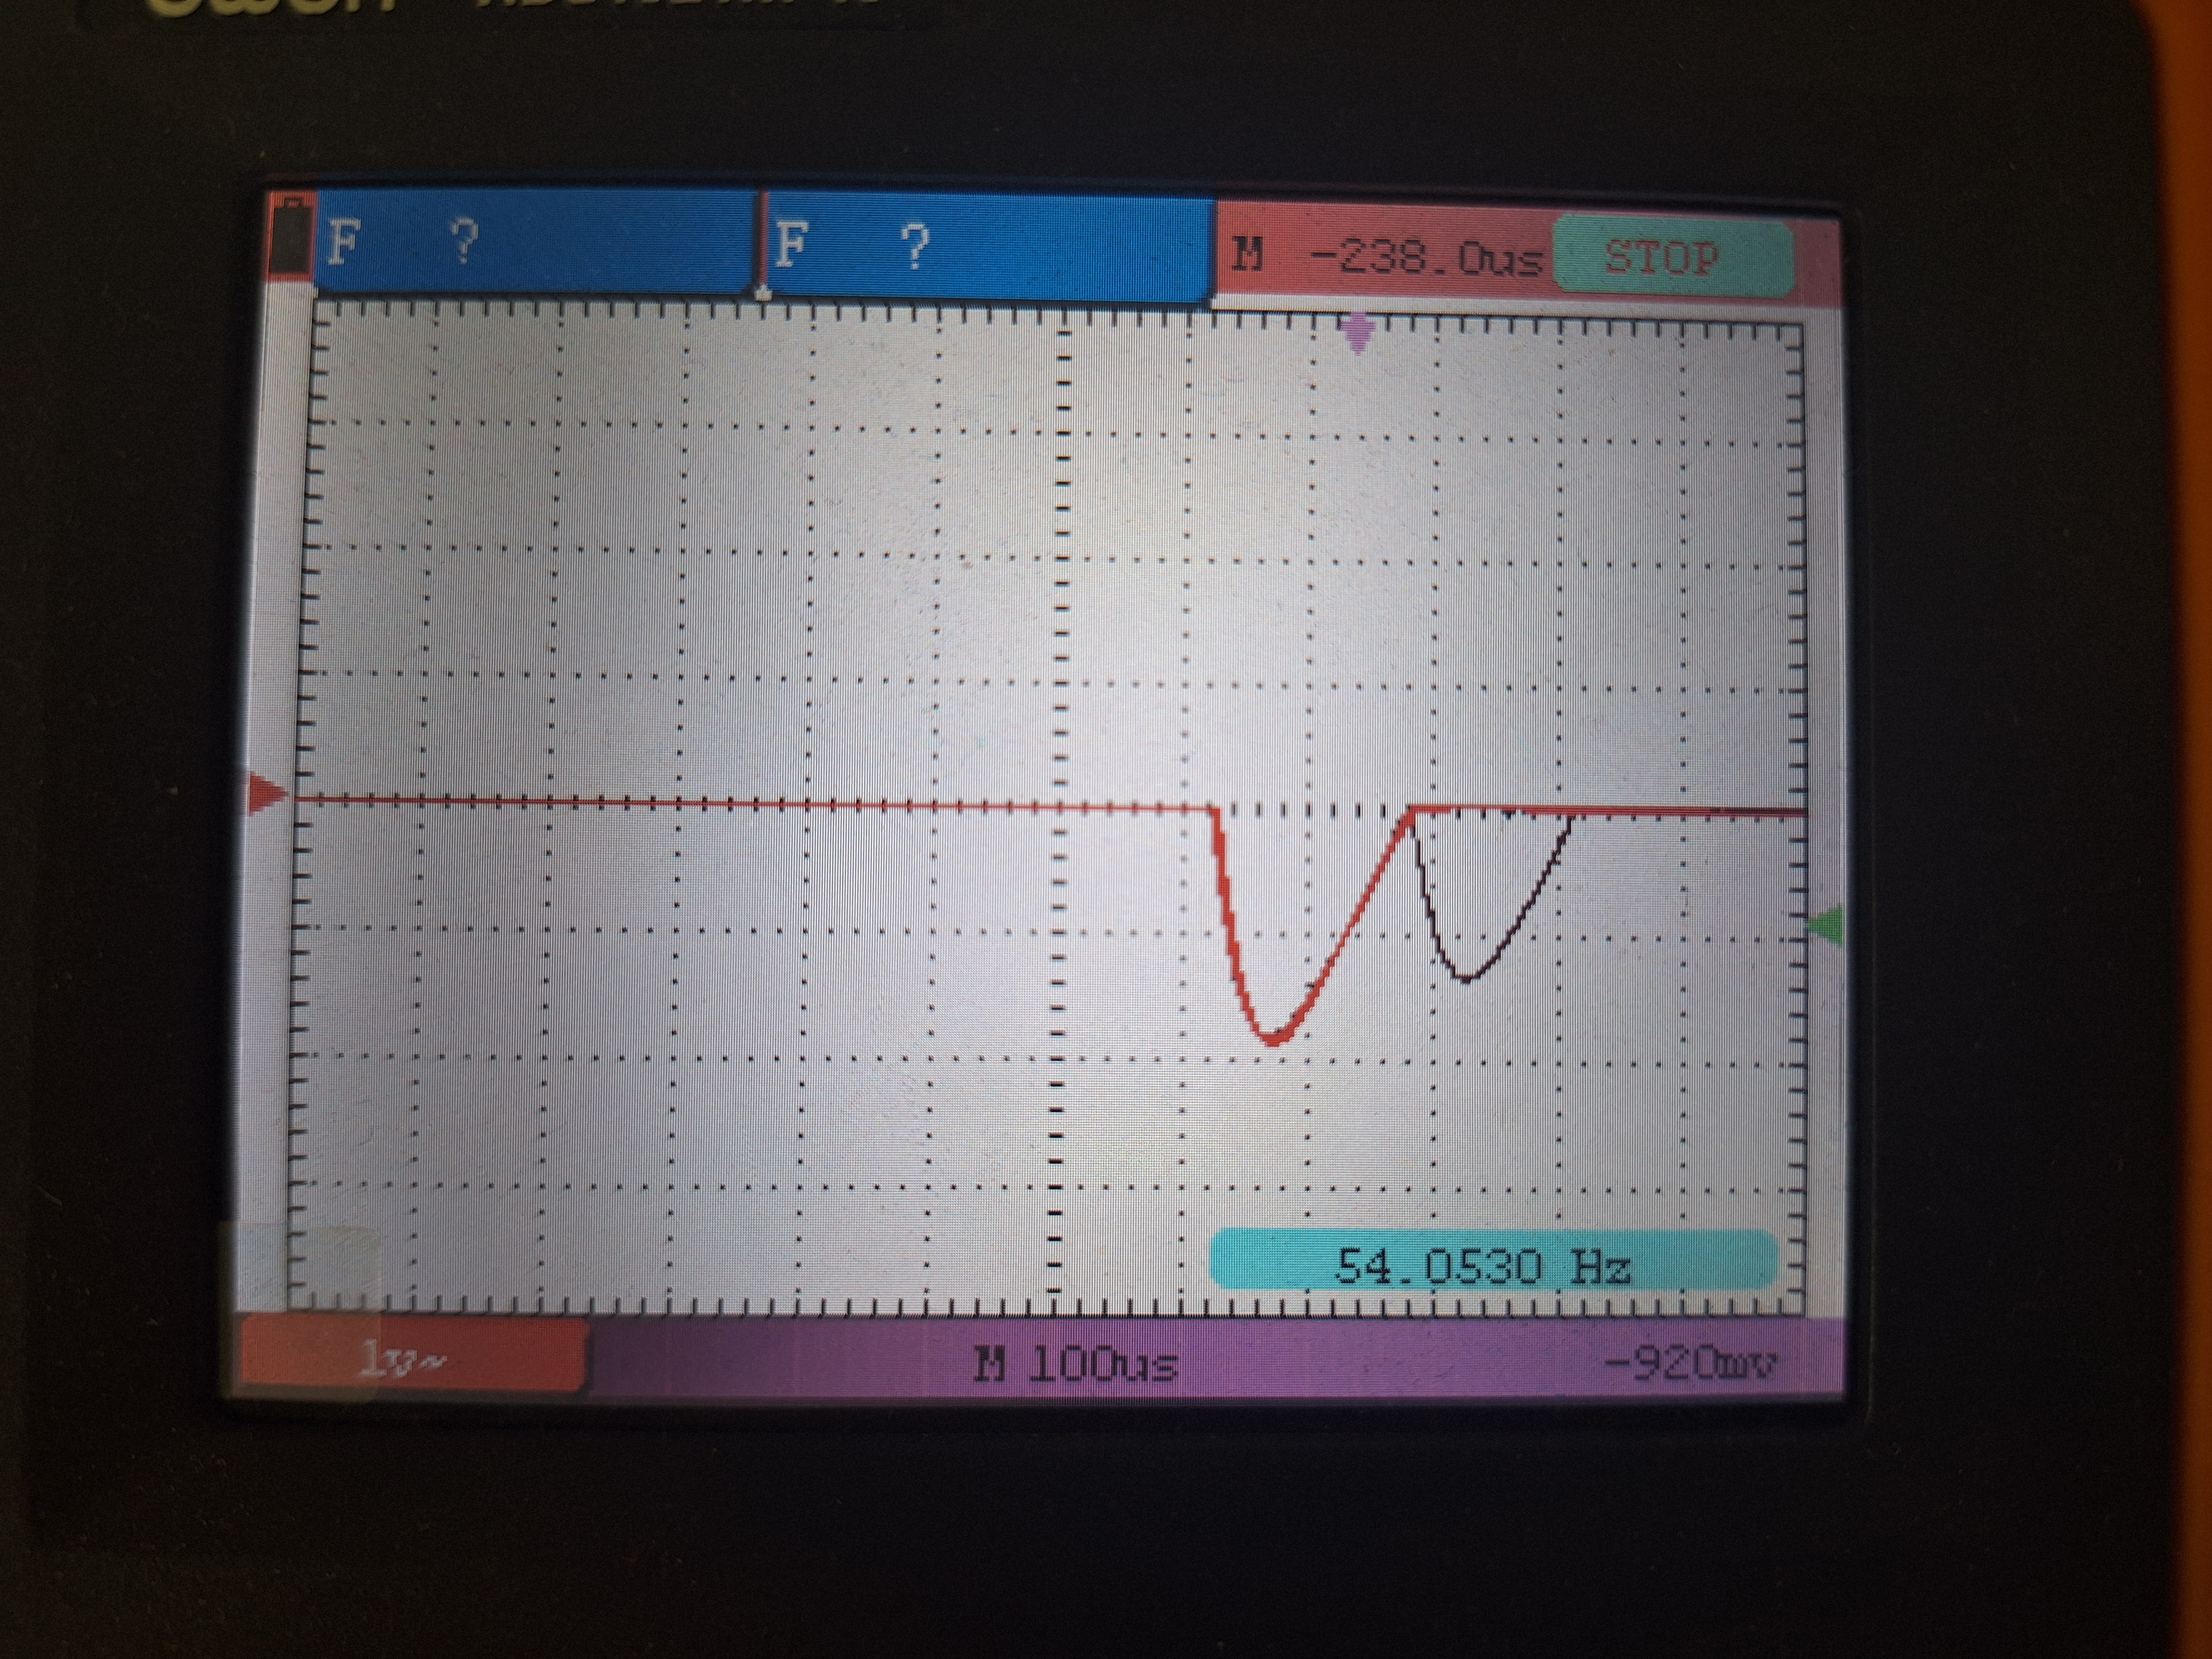
\includegraphics[width=0.8\textwidth]{Bilder/totzeit.jpg}
\end{figure} 

